%!TEX root = ../report.tex
\documentclass[../report.tex]{subfiles}
\begin{document}
    \chapter{State of the Art}

    \section{Explainability Vs Interpretability Methods}
    Use as many sections as you need in your related work to group content into logical groups
    \section{Taxonomy of Explainability Methods}

    \section{Explainability Methods for Neural Networks}
    \subsection{Types}
    \subsection{Choice of Methods for Further Evaluation}
    \subsubsection{Occlusion Sensitivity Maps}
    Occlusion sensitivity Mapping is a model-agnostic perturbation based method, which generates explanations by manipulating parts of the input image. The approach is computationally expensive, O(#simultaneous occlusions * #features * #ablations\_per\_eval * 1/#strides), and is included in this work to verify if Gestalt Matcher model is focusing on key facial features, or simply using the surrounding context to produce predictions. This is achieved by systematically occluding different portions of the input image with a black square or rectangular mask, and computing the difference in outputs (logit scores of the target class). In this work, we use a  black square mask of dimensions 10x10. Important portions of the input when occluded, result in relatively larger logit score differences, than the trivial ones. The differences are plotted on the image, yielding the occlusion sensitivity maps.     
    \begin{figure}[ht!]
    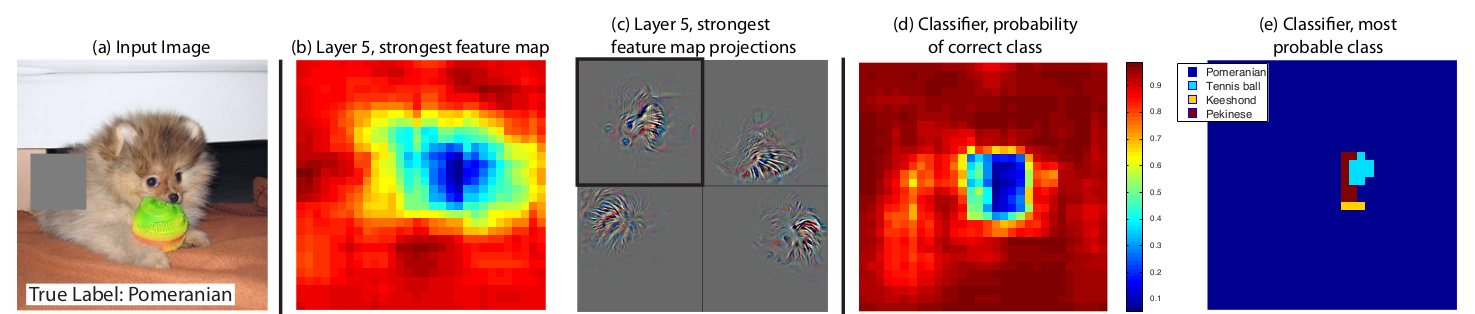
\includegraphics[width=\textwidth]{images/occlusion_sensitivity_map}
    \caption{An illustration of occlusion sensitivity mapping. Source: \cite{zeiler2011adaptive}}
    \label{osm}
    \end{figure}
    
    \subsubsection{Deconvolution}
    Zeiler and Fergus proposed the \enquote{Deconvolution} approach to visualize and provide insights into the functions learned by intermediate layers of a CNN. It is one of the earliest attribution techniques, which produces visualizations based on computing gradient of loss function with respect to a given input. The work acts a baseline till date for development and evaluation of new pixel attribution techniques.\\
    The method uses a deconvolution counterpart for every building block of a CNN, to obtain reverse mapping from features to input pixels. The idea of deconvolution was first introduced by Zeiler et al. \cite{zeiler2011adaptive}, as a way to perform unsupervised learning. In order to obtain attribution maps using the Deconvolution approach, the first step is to attach each block of convnet with its deconvolution counterpart as shown in the figure 1. Every activation except the ones belonging to the class of interest is set to zero. The activation value is then backpropagated through the deconvolution blocks such as unpooling, rectification and transposed convolution, all the way to the input layer. Deconvolution blocks act according to a pre-defined set of rules. The transposed convolution block performs the inverse of convolution operation by using transposed versions of the same filters. This is equivalent to flipping a given filter both in vertical and horizontal directions. In order to backtrack activations through max-pooling layer (.i.e. using the unpooling layer), indices corresponding to maximum activations in every layer, are first stored during the forward pass and later retrieved during the back propagation phase. However, the use of indices or switches from the forward pass, constrains the visualization on the input image \cite {guided_backprop}.\\ 
    Authors test their method on an AlexNet \cite{} trained on the ImageNet \cite{krizhevsky2012imagenet}, Caltech-101 \cite{} and Caltech-256 \cite{} and PASCAL2012 \cite{} datasets. As a first step, they visualize the top 9 feature maps of the each of the first five layers, to show the proportional increase of complexity in features with respect to their receptive fields. The visualizations are obtained by backtracking the strongest activation of a feature map for most of the data samples, all the way until a given input, using the deconvolution rules.The paper also discusses about the proportionality between the time taken for a given layer to learn features and its corresponding depth. Further, it shows that features learned by top layers are more invariant to transformations like translations, rotations and scale changes.\\
    The work evaluates itself by qualitatively comparing its resulting attribution maps with occlusion sensitivity maps. Occlusion sensitivity maps (\ref perturbation method) are obtained by systematically occluding portion of an image and analyzing the given classifier’s output, to determine the most discriminative regions as shown in the first image of Figure \ref{}.
    
    \subsubsection{Saliency Maps}
    Simonyan et al. propose two visualization techniques with intents to generate an image which maximizes the class score, and to compute a class-specific saliency map for a given input. The first technique numerically optimizes the input image while the other computes the spatial support of a given class in an input. This work is one of the earliest to leverage saliency maps for the task of weakly-supervised object segmentation. Authors demonstrate the proposed techniques by applying to a deep convnet trained on the ILSVRC-2013 dataset. \cite{ILSVRC15}
    
    \subsubsection{Class Model Visualization}
    The intention of this technique is to numerically generate an image which is representative of the target category with respect to the convolutional net’s class scoring model. This is achieved by finding a L2-regularised image such that the logit $S_{c}$  of a given class c is maximized:
    \begin{equation*}
        
    \end{equation*}
    
    where  $\lambda$ refers to the regularization parameter and I is a local optimum, which can be found with help of back propagation. The optimization process uses the mean image of the data set as the initial value. The work also mentions about the prominence of visualizations produced by using logit scores over soft-max/ un-normalized class scores.
\end{document}
